%
%	Praxisbezug
%

\pagebreak
\section{Data Analysis}

\onehalfspacing

\subsection{Blog Post Data Overview}

Before enriching the data for analysis, let's have a look at the raw web analytics data and KPIs for the various posts:

\begin{figure}[H]
\centering
\caption {Raw Blog Post Data}
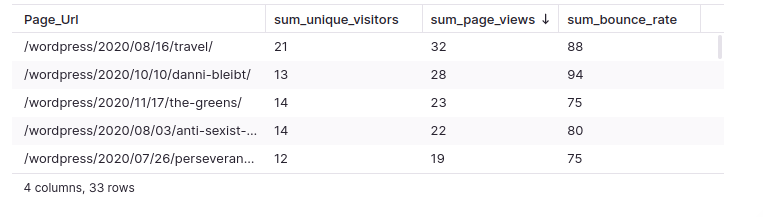
\includegraphics[width=\linewidth]{images/analysis-raw.png}
\label{fig:analysisRaw}
\end{figure}

I have excluded all top-level access, such as from "/wordpress/". Visits by accessing the blog itself and then scrolling down can unfortunately not be attributed to a certain post and thus not be enriched with category or sentiment data.

\subsection{Data Wrangling}

Adding category information from the blog to the raw blog post data from above was relatively easy and a straight-forward exercise with vi.

Text from blog posts on a WordPress blog, however, cannot easily be extracted. Wordpress offers an export function, but that will result in an archive in XML format, which is not suitable for text analysis.

After several tests, I found that the best way to extract the text from the actual posts was to use a text-based browser, such as Lynx, Links or Elinks; I chose Elinks for the task.

We already have the post URL in the blog post data above, so extracting was done with a simple shell script:

\verb|elinks https://.../2020/08/16/travel/ -dump > travel|

\verb|...|

As a the next step I created a small Python script to analyze the text and return the compound sentiment value:

\begin{lstlisting}[caption=Vader Sentiment Compound, frame=single, basicstyle=\ttfamily]
from vaderSentiment.vaderSentiment 
  import SentimentIntensityAnalyzer

analyzer = SentimentIntensityAnalyzer()

filenames = [ "anti-sexist-social-club",
              "biden-harris",
              ...
              "xfce" ]

for filename in filenames:
  fd = open(filename)
  blogPost = fd.read()
  sentiment = analyzer.polarity_scores(blogPost)
  print(filename + " " + 
    str(int(sentiment['compound'] * 10)))

\end{lstlisting}

This script will return the compound sentiment value for the blog post from the VADER analysis, one row per post.

\verb|anti-sexist-social-club 9|

\verb|biden-harris 6|

\verb|...|

\verb|xfce 9|

Adding the sentiment to the raw data again was a task for vi and sed.

As a result, we now have a data set of all blog posts, the associated KPI values, their categories and their sentiment.

\subsection{Blog Post Category Correlation}

Now that we've enriched the blog post data with category and sentiment information let's look at our KPIs by category. As a reminder, the encoding was as follows:

\begin{itemize}
\item Climate and politics: 1
\item Cloud: 2
\item Social Media and culture: 3
\item Covid-19: 4
\end{itemize}

\begin{figure}[H]
\centering
\caption {Category Analysis}
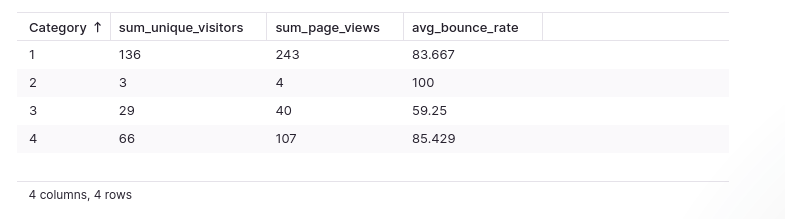
\includegraphics[width=\linewidth]{images/analysis-category.png}
\label{fig:analysisCategory}
\end{figure}

The top-performing category with the most unique visitors, the most page views, and the lowest bounce rate is Climate and Politics; the second-best performing category in all KPIs is Covid-19. The two other categories fall way behind - my posts regarding either Cloud or Social Media don't seem to be interesting to my readers.

\subsection{Blog Post Sentiment Correlation}

For the two best performing categories, Climate and Politics, and Covid-19, let's have a look at the KPIs broken down by sentiment, Climate first.

The sentiment is a compound value from the NLP analysis with ranges between -10 and 10, from a total negative to a total positive sentiment.

\begin{figure}[H]
\centering
\caption {Sentiment Analysis - Climate}
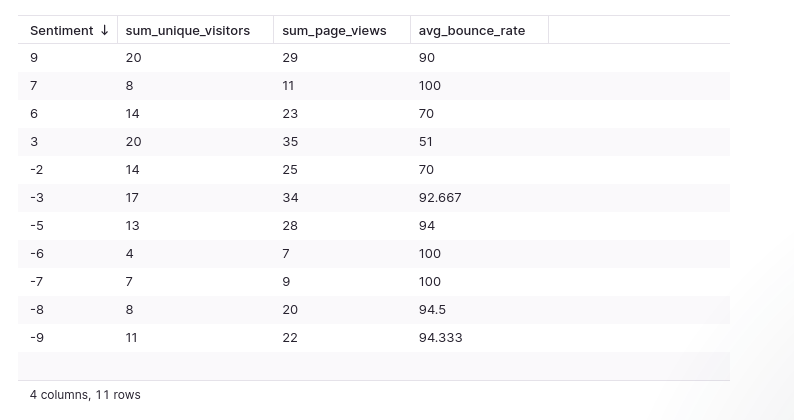
\includegraphics[width=\linewidth]{images/analysis-sentiment-climate.png}
\label{fig:sentimentClimate}
\end{figure}

If we compare the number of Unique Visitors for a Climate post with positive and negative sentiment, we cannot observe a significantly large difference (62 vs. 74). When we look at the number of Page Views (98 vs. 145), we can see a slight difference, with favor towards climate action posts with a more negative sentiment. There seems to be no influence from the posts' sentiment on the average Bounce Rate.

Now let's do the same analysis for posts regarding Covid-19 and the current pandemic.

\begin{figure}[H]
\centering
\caption {Sentiment Analysis - Covid-19}
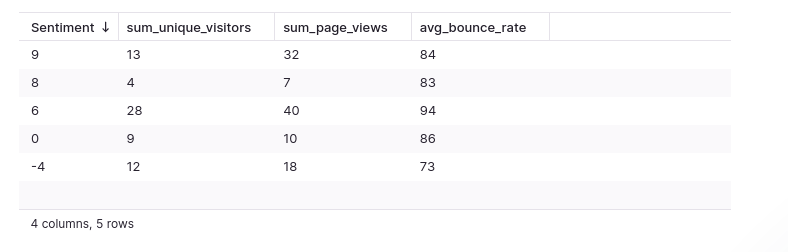
\includegraphics[width=\linewidth]{images/analysis-sentiment-covid.png}
\label{fig:sentimentCovid}
\end{figure}

Now there's a visible difference - both Unique Visitors (45 vs. 21) and Page Views (79 vs. 28) are significantly higher for blog posts on Covid-19 with a more positive sentiment. Again, there seems to be no influence from the posts' sentiment on the average Bounce Rate.

\subsection{Discarded graphs}

There were a couple of graphs that I discarded during analysis. I made an attempt to look at the blogs post's KPIs over time or by publish day, with no significant results. Equally uninteresting were my attempts to correlate data on the visitor's origins with the performance of the posts - I had hope for insights such as "Visitors from Austria as more interested im Climate Change than visitors from Switzerland' but alas, the data would offer no such hints.

\subsection{Results}

But there was enough information in the data to make the exercise worthwhile and yield a couple of actionable results:

\begin{itemize}
\item Focus on Climate, Politics, and Covid-19
\begin{itemize}
\item Focus on the dangers for climate change
\item Be upbeat about the outlook on Covid-19
\end{itemize}
\item Improve Google Search settings 
\item Remove Facebook referrals (maybe)
\item Switch to German language (maybe)
\item Improve access for mobile devices
\end{itemize}

\subsection{Outlook}

Coming back to the original question for the paper "On which subject(s) should I post to increase my reach?", we now have a definite answer.

According to the data, posting more content on Climate Change and Covid-19 should lead to more engagement from my visitors.

I'll keep that in mind for the future and change the content that I post accordingly.

\subsection{Data Source}

Again you can find the raw data and all charts from this chapter in the data notebook here: \href{https://count.co/n/CvJzzrqBsNI}{WTA Chapter 4}
